\documentclass[twoside,twocolumn]{article}

\usepackage{blindtext} 
\usepackage{graphicx}
\usepackage[sc]{mathpazo} 
\usepackage[T1]{fontenc} 
\linespread{1.05} 
\usepackage{microtype} 


\usepackage[english]{babel} 


\usepackage[hmarginratio=1:1,top=32mm,columnsep=20pt]{geometry} 
\usepackage[hang, small,labelfont=bf,up,textfont=it,up]{caption} 
\usepackage{booktabs} 


\usepackage{lettrine} 


\usepackage{enumitem} 
\setlist[itemize]{noitemsep} 


\usepackage{abstract} 
\renewcommand{\abstractnamefont}{\normalfont\bfseries} 
\renewcommand{\abstracttextfont}{\normalfont\small\itshape} 


\usepackage{titlesec} 
\renewcommand\thesection{\Roman{section}} % 
\renewcommand\thesubsection{\roman{subsection}} 
\titleformat{\section}[block]{\large\scshape\centering}{\thesection.}{1em}{} 
\titleformat{\subsection}[block]{\large}{\thesubsection.}{1em}{} 


\usepackage{fancyhdr} 
\pagestyle{fancy} 
\fancyhead{} 
\fancyfoot{} 
\fancyhead[C]{Titulo $\bullet$ Junio 2019 $\bullet$ } 
\fancyfoot[RO,LE]{\thepage} 


\usepackage{titling} 


\usepackage{hyperref} 


%----------------------------------------------------------------------------------------
%	TILULOS
%----------------------------------------------------------------------------------------


\setlength{\droptitle}{-4\baselineskip} 

\pretitle{\begin{center}\Huge\bfseries} 
\posttitle{\end{center}} 
\title{Business Intelligence and Business Analytics} 
\author{Andre Reinoso Aranda, Marko Antonio Rivas Rios, Andree Velasco Sucapuca, \\
Percy Taquila Carazas, Roberto Zegarra Reyes. }
\date{\today} 
\renewcommand{\maketitlehookd}{
\begin{abstract}
\noindent 
Business Intelligence BI is a tool, below different kind organizations, supports
decisions making processes, based in an exact and accurate information;
guarantying the production of the needed knowledge that lets to choose the most
appropiate option for the company success. The investigation begins with the BI
definition and applications; by addition shows definitions and relevant BI
investigations tools, like Data Warehouse, Olap, Balance Scorecard and Data
Mining.
\end{abstract}
\begin{abstract}
\noindent 

La Inteligencia de Negocios BI (Business Intelligence) es una herramienta bajo
la cual diferentes tipos de organizaciones, pueden soportar la toma de decisiones
basadas en información precisa y oportuna; garantizando la generación del
conocimiento necesario que permita escoger la alternativa que sea más
conveniente para el éxito de la empresa. La investigación comienza con la
definición y aplicaciones de BI; además se muestran trabajos relevantes en
algunas de las herramientas para hacer BI, como son Data Warehouse (Bodega
de Datos), Olap (Cubos Procesamiento Analítico en Línea), Balance Scorecard
(Cuadro de Mando) y Data Mining (Minería de Datos). 

\end{abstract}
}

%----------------------------------------------------------------------------------------

\begin{document}

% Print the title
\maketitle

%----------------------------------------------------------------------------------------
%	INTRODUCCION
%----------------------------------------------------------------------------------------

\section{Introduccion}
\lettrine[nindent=0em,lines=3]{A}ctualmente en el Perú las pequeñas y medianas empresas producen al mercado peruano ingresos y empleo, la gran cantidad de informacion que manejan es debido al alto numero de operaciones que realizan a diario.\\ \\
El aumento de competencia hace que el area administrativa tome decisiones a base de su experiencia, publicidad, tecnologia, recursos humanos y hasta de su propia intuicion.\\ \\
Sin embargo hay empresas que no toman de manera estructurada las decisiones, o no implementan herramientas de Business Intelligence que permitirian al gerente escenarios, reportes, etc. una mejor toma de deciciones respecto a su rubro. \\ \\
Aquella empresa que si lleva a cabo procesos de extraccion de datos, transformacion de datos, uso de herramientas y metodos, tendra una ventaja notoria a comparacion de las demas que no lo aplican.
\\ \\
El Business Analytics busca trabajar los datos con conceptos estadisticos, modelos analiticos, permitiendo la elaboracion de escenarios con las que las organizacion tomen decisiones anticipandoce a lo que vendra a futuro. El Business Analytics busca la simulacion de procesos, el desarrollo de escenarios, predicciones, relaciones entre las areas de una organizacion, etc.


%----------------------------------------------------------------------------------------
%	Objetivos
%----------------------------------------------------------------------------------------


\section{Marco teorico}

\begin{itemize}
\item Inteligencia de Negocios (BI): \\ 
Inteligencia de Negocio se refiere al proceso de
convertir datos en conocimiento y conocimiento en
acciones para crear la ventaja competitiva del
negocio. 
\begin{center}
	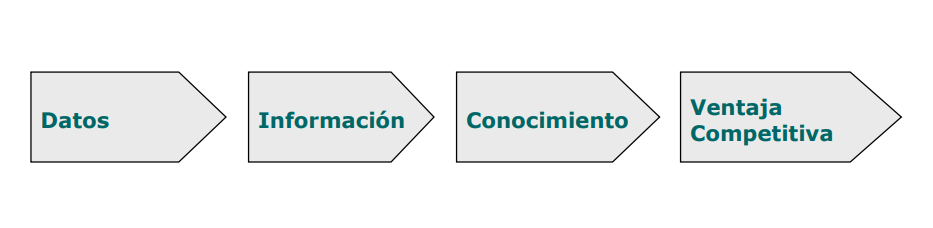
\includegraphics[width=7cm]{./Imagenes/bi} 
\end{center}

\item Ventajasde la Inteligencia de Negocios: \\
La Inteligencia de Negocios
tiene como función suministrar toda la información necesaria para la toma de
decisiones de un negocio, organización o empresa. Dependiendo de la misión de
la empresa, la Inteligencia de Negocios permite proporcionar toda la información
relacionada a esta, ya sea de sus clientes, sus procesos, sus tareas,
competencias o para predecir cambios o movimientos posteriores. 
todas las empresas tienen la posibilidad de
transformar sus datos en información por medio de herramientas de Inteligencia
de Negocios (o Business Intelligence), que logran un camino oportuno hacia la
toma de decisiones. Por lo Tanto : \\ \\ 


	\item Permite integrar datos de diferentes fuentes o áreas de la empresa, y acceder
a esta información a través de un formato único. \\
  
	\item Aporta la información basada en tiempo y hechos reales, distribuyéndola en
toda la organización y para los diferentes actores de la misma. \\


	\item Las herramientas ofrecidas por Business Intelligence, permiten una fácil y
rápida interacción con los usuarios, además de mostrar la información a gran
velocidad. \\

	\item Permite que la empresa tenga un continuo seguimiento de sus procesos, para
tener las mejores y acordes visiones de la empresa a largo plazo.\\


\item Arquitectura de una solución de Inteligencia de Negocios: \\


Una solución de Business Intelligence parte de los sistemas de origen de una organización
(bases de datos, ERPs, ficheros de texto...), sobre los que suele ser necesario
aplicar una transformación estructural para optimizar su proceso analítico.

A partir de las fuentes de datos generadas en las organizaciones, se procede con
una fase de extracción, transformación y carga,

La información transformada o modificada, es almacenada en un Data Warehouse
o Repositorio de datos, en donde es posible administrar y monitorear los procesos
o consultas del sistema, y que a la vez está relacionado con la construcción de
Data Marts, es decir, son estructuras enfocadas al análisis de los datos a partir de
bases de datos transaccionales o analíticas, y dirigidas a áreas específicas de una
empresa u organización. 

Todos los datos almacenados se exploran a partir de herramientas de
visualización de la información, las cuales permiten el desarrollo de reportes,
análisis, cuadros de mando, alertas, y diferentes instrumentos que se llevan hasta
los usuarios para dar soporte a sus decisiones y así proporcionar soluciones de BI
mucho más completas.\\

el modelo integral o esquema de una solución de
Inteligencia de Negocios está compuesto por: \\


- Diseño Conceptual. Que comprende aspectos ligados a la estructura de la
información que se encuentran en las diferentes fases de la solución, ya sea los
objetivos, la misión, los indicadores clave de rendimiento, los modelos, o todos los
requerimientos necesarios para la construcción e implementación de la misma. \\

- Construcción de los Data Marts y Data Warehouse. Es importante
conocer las fuentes de datos y hacer los procesos de extracción, transformación y
carga, para tener dichos datos de una forma estructurada, seleccionada y
unificada. Por lo tanto, “no diseñar y estructurar convenientemente y desde un
punto de vista corporativo el DataWarehouse y los Datamarts generaraan problemas
que pueden condenar al fracaso cualquier esfuerzo posterior: información para la
gestión obtenida directamente a los sistemas operacionales, florecimiento de
Datamarts descoordinados en diferentes departamentos, etc”  \\

- Herramientas de explotación y exploración de la información. Se
identifican las herramientas funcionales y acordes a la solución. Dichas
herramientas permiten la elaboración de reportes e informes a partir de la
información generada en los Data Warehouse, Cuadros de Mando para el análisis
rápido de resultados y presentación de los indicadores, y Análisis en línea
teniendo en cuenta las bases de datos relacionales y los modelos generados. \\




\end{itemize}



%----------------------------------------------------------------------------------------
%	DESARROLLO
%----------------------------------------------------------------------------------------

\section{Desarrollo}

\subsection{¿Que es la inteligencia de negocios?}

La informacion ha propiciado la necesidad de tener mejores, mas rapidos y mas eficientes metodos para extraer y transformar los datos de una organizacion en informacion.
\\ \\
En 1958 \textbf{Hans Peter Luhn}, investigador de la IBM, acuña el termino en el articulo "A Business Intelligence System":
\\ \\
\textsl{''La habilidad de aprender las relaciones de hechos presentados de forma que guien las acciones hacia una meta deseada'' (Hans Luhn, 1958)} \\ \\

 \textbf{ ¿Como funciona el sistema?}

\textsl{''Este sistema de inteligencia utilizará el procesamiento de datos para la auto-abstracción y auto-codificación de documentos y para crear perfiles de interés para cada uno de los "puntos de acción" en una organización.'' (Hans Luhn, 1958)}
\\ \\

En 1989 \textbf{Howard Dresden}, analista de Gartner, propone una definicion formal del concepto.
\\ \\
\textsl{"Conceptos y métodos para mejorar la toma de decisiones comerciales mediante el uso de un sistema de soporte basado en hechos''}
\\ \\
En pocas palabras: \\ \\
\textbf{Es el conjunto de metedologias, aplicaciones, capacidades administrativas de informacion que permite tomar mejores decisiones a los usuarios de una organizacion.}


\subsection{¿Cuando aplicar la inteligencia de negocios?}

Contenido

\subsection{¿Qué ventajas nos da usar la inteligencia de negocios?}

- Nos permite tomar decisiones rápidas. \\
- Ayuda a definir escenarios adecuados. \\
- Permite tomar la información, la convierte en conocimiento para la toma de decisiones. \\
\subsection{Beneficions de la inteligencia de negocios}

- Beneficios tangibles, por ejemplo: reducción de costes, generación de ingresos, reducción de tiempos para las distintas actividades del negocio. \\\\
- Beneficios intangibles: el hecho de que tengamos disponible la información para la toma de decisiones hará que más usuarios utilicen dicha información para tomar decisiones y mejorar la nuestra posición competitiva, por ejemplo: Cuales son los horarios en que más visitan la tienda, cual es el recorrido que hacen en el interior del local. \\\\
- Beneficios estratégicos: Todos aquellos que nos facilitan la formulación de la estrategia, es decir, a qué clientes, mercados o con qué productos dirigirnos, por ejemplo: ofertas que más solicitan los clientes. \\\\

\subsection{¿Que es el análisis de negocio?}

Es la exploración iterativa y metódica de los datos de una organización, resaltando el análisis estadístico. El análisis empresarial es usado por empresas que toman decisiones basadas en datos. 
\\ \\
Las empresas basadas en datos tratan sus datos como un activo corporativo y buscan convertirlos en una ventaja competitiva. El análisis empresarial depende de la calidad de los datos, de los analistas expertos que entienden las tecnologías y el negocio, y el compromiso de la organización de utilizar los datos para obtener información que ayude en las decisiones comerciales.
\\ \\
Bussiness analytics, se define como el campo del análisis empresarial, se trata del proceso de recopilación, almacenamiento y análisis de datos para asesorar a una empresa mejorando su eficiencia para aumentar sus ingresos.
\\ \\
Si una empresa usa un enfoque que se base en datos en su proceso de toma de decisiones, da como resultado que el análisis juega un rol de gran importancia para la toma de decisiones.  Las personas especialistas en este tema se llaman \textbf{ “Analistas Empresariales”}
\\ \\
Las instituciones recopilan y almacenas datos durante muchos años, pero en los últimos años, han aumentado en cantidad significativa pero la mayor parte de estos datos no están estructurados.  
\\ \\

\textsl{“Según MarTech, el universo digital tiene 2,7 Zettabytes de datos, y si la mayor parte no está estructurada, analizarlo requerirá muchos analistas de datos.  No es de extrañar que el gasto en proyectos de bigdata (proyectos de análisis de negocios) en el 2018 alcanzó los \$114 mil millones de dólares."} (Noodle Staff,2018)

\subsection{Función del análisis de negocio}
Cuando se determina el objetivo comercial del análisis, se selecciona una metodología de análisis y se adquieren datos para respaldar dicho análisis.  Esta adquisición de datos implica la extracción de uno o más sistemas comerciales, la limpieza y la integración en un único almacén de datos.
\\ \\
Este análisis inicial se realiza con una muestra pequeña de datos.  Las herramientas que se utilizan van desde hojas de cálculo, estadística, aplicaciones complejas de extracción de datos y modelado predictivo. A medida que se van descubriendo patrones y relaciones, se hacen nuevas preguntas, completando el proceso analítico, hasta que se cumpla el objetivo comercial.
\\ \\
El despliegue de modelos predictivos implican la puntuación de registros de datos, generalmente en una base de datos, el uso de los puntajes son para optimizar las decisiones en tiempo real, dentro de las aplicaciones y los procesos comerciales del BA, además ayuda en la toma de decisiones tácticas en respuesta a eventos imprevistos.  Y en muchos casos, hasta la toma de decisiones esta automatizada para admitir respuestas en tiempo real.
\subsection{Tipos de análisis de negocio}
Los tipos específicos de análisis de negocios incluyen (Rouse, 2019):


\begin{itemize}	

	\item \textbf{Análisis descriptivo}: Rastrea los indicadores clave de rendimiento (KPI) para comprender el estado actual de un negocio.
	\item \textbf{Análisis predictivo}: Analiza los datos de tendencias para evaluar la probabilidad de resultados futuros.
	\item \textbf{Análisis prescriptivo}: Utiliza el rendimiento pasado para generar recomendaciones sobre cómo manejar situaciones similares en el futuro.

\end{itemize} 

\subsection{Aplicaciones de análisis de negocio}
Las herramientas de análisis de negocio vienen en varias variedades diferentes (Rouse, 2019):
\begin{itemize}	

	\item Herramientas de visualización de datos
	\item Plataformas analíticas de autoservicio
	\item Herramientas de análisis estadístico
	\item Software de informes de inteligencia empresarial
	\item Plataformas de Big Data

\end{itemize} 


%----------------------------------------------------------------------------------------
%	CONCLUSIONES
%----------------------------------------------------------------------------------------

\section{Conclusiones}
\begin{itemize}	

	\item  En el mundo empresariial, las empresas tienen un area que brinda soporte a los procesos de informacion, estrategia, lo que los lleva a un mercado competitivo, la inteligencia de negocios para una empresa la hace una pieza fundamenta a la hora de tomar mejores deciones.
	\item El numero creciente de pequeñas y medianas empresas da una notoria cifra sobre la ausencia de un sistema de inteligencia empresarial para la gestion de sus empresas. Pero en contraste si tienen conocimiento del concepto y de sus beneficios como el del acceso a datos criticos de la empresa, oportunidades competitivas, tomar mejores deciciones, etc.
	\item Lo que buscan estas herramientas es fomentar la exploración de datos y la toma de decisiones basadas en hechos.
	\item El Business analytics busca prodocir conocimiento estadisticoos y matematicos a partir de datos, con el objetico de generar probales escenarios y opciones con las que lidiar, a comparacion del Business Intelligence que proporciones un analisis a base de datos historicos

\end{itemize} 



%----------------------------------------------------------------------------------------
%	BIBLIOGRAFIA
%----------------------------------------------------------------------------------------


\begin{thebibliography}{99} 

\bibitem[Silvia Chavez y Carmen Contreras, 2018]{}
\newblock Implementación de Business Intelligence, para el proceso de toma de decisiones del área de ventas.

\bibitem[Hans Peter Luhn 1958]{}
\newblock A Business Intelligence System

\bibitem[Alex Rayón, 2015]{Universidad de Deusto}
Conceptos básicos del Business Intelligence.

\bibitem[Jordi Conesa y Josep Curto, 2010]{}
\newblock Introduccion al Business Intelligence

\bibitem[Margaret Rouse, 2019]{}
\newblock Análisis de negocios (BA)

\bibitem[Noodle Editorial Staff, 2018]{}
\newblock Business analytics career paths

\bibitem[Josep Lluis Cano, 2007]{}
\newblock Business Intelligence: competir con información
 

 
\end{thebibliography}


%----------------------------------------------------------------------------------------


\end{document}
